\section{BACKGROUND}

Several IPC systems that are commonly used today were researched and evaluated. Sockets was evaluated utilizing UDP, TCP, and ZeroMQ. THe ACH library was used for an example of shared memory. The details of their use and implementation are presented in the following.

\subsection{Shared Memory (ACH)}

Shared memory offers the fastest read/write speeds for communication between processes within a single computer. As part of the POSIX\footnote{POSIX: Portable operating system interface. A set of standards for maintaining compatability between opearting systems.} IPC library, shared memory is available to virtually every robotic system. Real time robotics require that the IPC system be able to prioiritize the most recent data over data received sequentially (non head of line blocking). Basic shared memory provides this by overwriting variables but is susceptable to synchronization issues and all previous data is now lost\cite{REALTIMEACH}. 

ACH\footnote{Available at https://github.com/golems/ach} builds on basic shared memory and provides a message bus (channel) between mutliple writers and multiple readers. An ACH channel consists of a data buffer and an index buffer that are stored in a shared memory file. The channel provides synchronized access via a mutex and a condition variable. This allows for priority inhereitence and prevents starvation\cite{REALTIMEACH}. The ACH library is open source and formally verified\cite{REALTIMEACH} making it suitable for widespread use.

ACH channels provide high levels of flexibilty in communication and programming. They can be configured to read the most recent data or in order it was received. A read command can block until data is received or it can poll the channel as needed. Figure \ref{fig:ach diagram} below is an example of an ACH based control system for the Hubo robot. 

\begin{figure*}[tbhp]
 \centering
 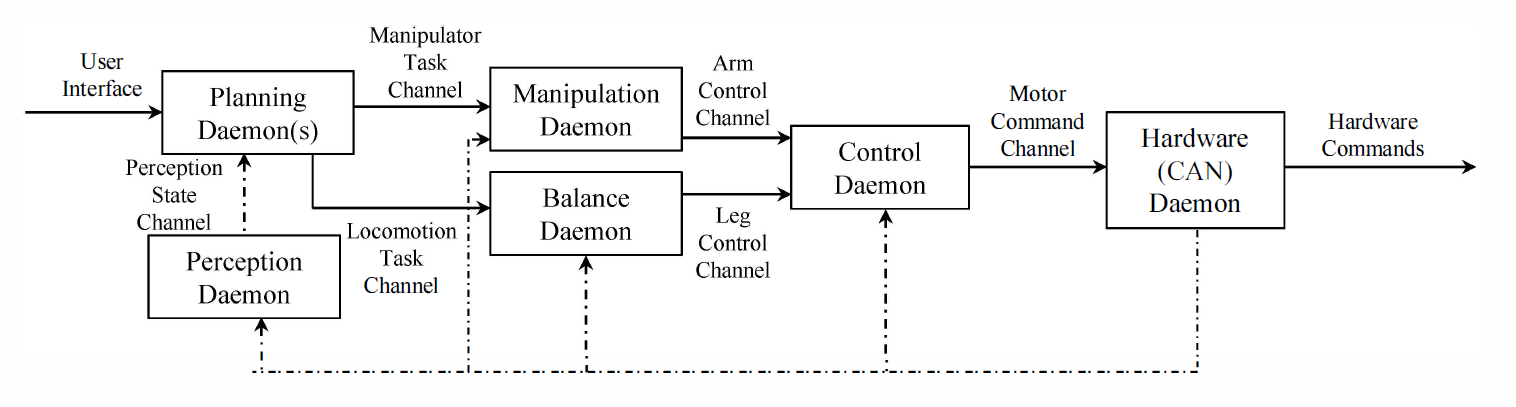
\includegraphics[width=2.0\columnwidth]{./images/achflow.png}
  \caption{ACH Communication Flow Chart for HUBO Robot\cite{REALTIMEACH}. Diagram shows control daemons used and communication paths used in the HUBO humanoid robot. Multiple publishers and subscribers for each channel show flexibility of implemenation.}
  \label{fig:ach diagram}
\end{figure*} 

ACH provides LAN based communications by utilzing sockets messages to transport channel data. Each system running the ACH network daemon (ACHD) can write directly to remote shared memory resources connected to the network\cite{ACHHUBO}. This allows for CPU intensive processes to be offloaded from the robot to a local high performance computer. 

\subsection{Sockets: TCP and UDP}

Sockets provides interprocess communication over a network via the TCP (Transmission Control Protocol) and UDP (User Datagram Protocol). It is built it to most operating systems which makes code highly portable. Sockets communicate with a client/server architecture with either point to point or multicast messages\cite{UDPMULTICAST}. Utilzing IP addresses and existing internet infrastructure allows processes to communicate with remote locations. This makes it possible to quickly and cheaply connect the robot to sensors, controllers, and embedded systems. As part of the POSIX library, sockets allows many different operating systems and programming languages to communicate with no extra software. Modern newtork routers offer gigabit connections enabling sockets to provide fast communication between distrubted processes.

Sockets message buffers are head of line blocking and disregard new messages when full. This is problematic for robotics where sensor data is of critical importance. 

\subsubsection{TCP}

TCP offers robust messaging between a single client and a single server process. Initial handshaking is required during connection and can cause additional latency for the initial message\cite{UDPTCP}. Each message transmission triggers a response from the recipient. This allows TCP to identify dropped messages and retransmit. While good for data integrity, response messages and retransmission increase latency. 

\subsubsection{UDP}

UDP offers one quick directional communication between processes. UDP supports client/server and multicast topologies. Processes are bound to IP address(s) and port number(s)\footnote{Multiple IP addresses and port numbers only available for a multicast UDP socket}. There is no handshaking or direct link between the processes. This allows mutltiple clients to send data to a single server. UDP inherently has less latency than TCP due its 'fire and forget' approach to messaging. Data integrity suffers as there is no way to identify missed messages. This method favors transmission speed and has less latency than TCP.

\subsection{Sockets: ZeroMQ}

ZeroMQ\footnote{Available at www.zeromq.org} (ZMQ) is a messaging system that extends on the foundations of sockets. It provides additional functionality to TCP by sending messages to a system topology instead of specific IP addresses. ZMQ prevents sending to specific IP addresses by design. The available messaging patterns is open ended. Common patterns include publish/subscribe and request/reply. Figure \ref{fig:zmq top} below shows examples of how toplogies can be arranged.

\begin{figure}[thpb]
 \centering
 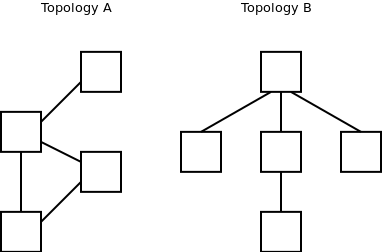
\includegraphics[width=1.0\columnwidth]{./images/zmqtopology.png}
  \caption{ZeroMQ Example Topologies\cite{ZMQTHEORY}. Figure shows two example topologies that can be implemented with ZeroMQ. Publishers are shown sending data to subscribers with multiple paths.}
  \label{fig:zmq top}
\end{figure} 

Only one messaging pattern is allowed for a topology and they cannot be interconnected. This guarentees that data will arrive at their intended location(s). ZMQ separates its stack into end to end and hop by hop layers. Unlike TCP/IP, each ZMQ end to end protocol has its own hop by hop protocol\cite{ZMQTHEORY}. This allows each specific messaging pattern to have their own routing functionality. Bidirectional messages can be sent to specific nodes in the topology. Each intermediary node can determine if downstream sections of the network are unreachable and can signal the original client to resend now or wait until connectivity has been reestablished. 

ZMQ provides synchronization for data in multithreaded applications. This functionality is hidden from the developer and allows for complex, scalable messaging in multithreaded systems. Common methods for dealing with synchronization (mutex locks, etc) can block threads when scaled to high number of processes. ZMQ absracts complex lock free synchronization methods behind the familiar interface of sockets\cite{MULTITHREADZMQ}.

\subsection{ROS}

ROS\footnote{Available at www.ros.org} (Robot Operating System) is a flexible framwork for developing robotic systems. Offering more features than an IPC, ROS utilizes TCP as its core transport mechanism for communication between processes. In addition to the IPC, ROS offers a wide library of prebuilt tools and a vast user base from which to draw on modular solutions that can plug into any ROS system. This reduces development time and amount of low level code that needs to be written for each piece of hardware. Figure \ref{fig:ROS Network Diagram} below shows an example ROS network diagram.

\begin{figure}[thpb]
 \centering
 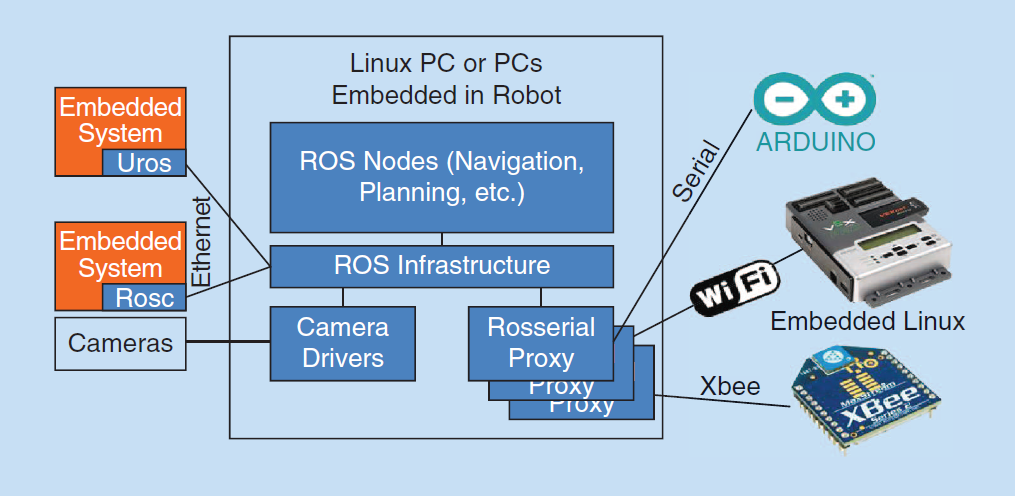
\includegraphics[width=1.0\columnwidth]{./images/rosnet.png}
  \caption{ROS Example Network Diagram\cite{EMBEDDEDROS}. Network diagram shows how a ROS system can be setup to incorporate a wide variety of off the shelf hardware and the internal processes the robot would need for communication.}
  \label{fig:ROS Network Diagram}
\end{figure} 

Commerically available embedded systems can interface with the ROS system by adding interface processes (ROS topics) to the core system. ROS was designed to support higher level robot functions instead of the control of individual motors/sensors/etc. Integration of subsystems is left to the designer as ROS does not support fieldbuses\cite{EMBEDDEDROS}. ROS can be implemented as a combination of an embedded PC, properietary systems with custom interfaces, and ROS Messaging. Embedded PCs provide smooth ROS integration but fail to offer hard real time support. Existing robots can be managed from ROS through topics acting as translators. This abstracts the lower level programming and allows for the existing systems to operate in real time. The IPC system for ROS operates on remote procedure calls and publish/subscribe protocols for messaging. 

The ROS IPC system allows for custom messages interface with embedded systems. Rosserial, rosc, and Rosbridge are methods of passing these messages. Rosserial provides a proxy over a C++ client that can be ported to any system that supports the language. Rosserial provides a ROS-like API to publish, subscribe, offer and consume RPC services over serial. The proxy can act as a bottleneck increasing message latency. Rosc allows for direct connection and messaging to systems supporting C, but TCP/IP overhead can overwhelm low level peripherals. Rosbridge allows dynamic socket and websocket access to the full capabiliies of ROS\cite{EMBEDDEDROS}.







